\chapter{Preliminary Design and Planning}
This chapter turns the proposal of the first two chapters into a first design. It lists what the system must do and how well it must do it, shows how a user works with it and how the data flows at run time, describes the preliminary architecture and the tools, and closes with the project timeline and the risks. The design is preliminary. It records the decisions taken so far and will be refined when the systematic recordings begin.

\section{Functional Requirements}
The functional requirements follow from the objectives in Chapter~1. Each requirement names the objective it serves, so that later chapters can report against it. Table~\ref{tab:fr} lists them.

{\small
\setlength{\tabcolsep}{4pt}
\begin{longtable}{L{1.1cm}L{10.6cm}L{1.9cm}}
\caption{Functional requirements}\label{tab:fr}\\
\toprule
\textbf{ID} & \textbf{Requirement} & \textbf{Objective}\\
\midrule
\endfirsthead
\multicolumn{3}{l}{\small Table \thetable\ (continued)}\\
\toprule
\textbf{ID} & \textbf{Requirement} & \textbf{Objective}\\
\midrule
\endhead
\bottomrule
\endfoot
FR1 & The transmitter shall send packets at a fixed, configurable rate. & 2\\\addlinespace
FR2 & Each receiver shall read the CSI of every packet it receives from the transmitter and forward it to the computer. & 2\\\addlinespace
FR3 & The computer shall read the three receiver streams at the same time, add a time stamp and the identity of the link to every packet, and store the raw data of a session in a file. & 2\\\addlinespace
FR4 & The operator shall be able to start and stop a recording session and to attach a label to it: the activity, the zone, the participant code and the room layout. & 2, 6\\\addlinespace
FR5 & The system shall learn an empty-room baseline for every link from a short calibration recording. & 3\\\addlinespace
FR6 & The system shall decide for every time window whether the room is empty or occupied by a moving person. & 3\\\addlinespace
FR7 & When no movement is found, the system shall search the signal for a breathing pattern and report a person who is present but still. & 4\\\addlinespace
FR8 & The system shall combine the three links into an approximate zone of the movement and a direction of movement. & 5\\\addlinespace
FR9 & The system shall extract features from every window and train a lightweight classifier on the labelled sessions. & 6\\\addlinespace
FR10 & The system shall evaluate every learned model on complete sessions that were not used for training and report accuracy together with the confusion between classes. & 7\\\addlinespace
FR11 & The system shall show the current state on a live display: empty or present, moving or still, zone and direction. & 3 to 5\\\addlinespace
FR12 & The system shall export the results of an evaluation so that they can be repeated and included in the report. & 7\\
\end{longtable}
}

\section{Non-Functional Requirements}
The non-functional requirements describe the qualities that the system must have besides its functions. Several of them come directly from the research gap in Section~\ref{sec:gap}: the hardware must stay cheap, the results must be honest, and the privacy of the people in the room must be respected. Where a number is given it is a target for the design. The values that are finally reached will be measured and reported.

{\small
\setlength{\tabcolsep}{4pt}
\begin{longtable}{L{1.3cm}L{2.7cm}L{9.6cm}}
\caption{Non-functional requirements}\label{tab:nfr}\\
\toprule
\textbf{ID} & \textbf{Quality} & \textbf{Requirement}\\
\midrule
\endfirsthead
\multicolumn{3}{l}{\small Table \thetable\ (continued)}\\
\toprule
\textbf{ID} & \textbf{Quality} & \textbf{Requirement}\\
\midrule
\endhead
\bottomrule
\endfoot
NFR1 & Low cost & The sensing hardware consists only of commodity Wi-Fi devices. No special radio equipment is needed.\\\addlinespace
NFR2 & Packet rate & Every link should deliver CSI at a steady rate close to the transmission rate of about 100 packets per second.\\\addlinespace
NFR3 & Responsiveness & The live display should follow a change in the room within a few seconds. The exact delay depends on the window length and will be measured.\\\addlinespace
NFR4 & Honest evaluation & No window of a test session may appear in the training data. Results are reported per session and also after a change of the room layout or of the device placement.\\\addlinespace
NFR5 & Robustness & A lost packet, a burst of interference or a receiver that is unplugged must not stop the recording. Windows with too few packets are marked and left out of the decision.\\\addlinespace
NFR6 & Short set-up & Installing the system in a new room should need only the placement of the devices and a short recording of the empty room.\\\addlinespace
NFR7 & Reproducibility & The device settings, the data format, the placement of the devices and the processing parameters are documented so that the set-up can be repeated by others.\\\addlinespace
NFR8 & Privacy & Recordings of people are made only with their consent. The stored data contain CSI values and labels, and no names, images or sound.\\\addlinespace
NFR9 & Lightweight processing & The detection and the classifier must run in real time on an ordinary laptop without a graphics card.\\\addlinespace
NFR10 & Maintainability & Acquisition, pre-processing, detection, fusion and evaluation are separate modules, so that one method can be replaced without changing the others.\\
\end{longtable}
}

\section{Use Case Diagram}
Figure~\ref{fig:usecase} shows the use cases of the system. There are two actors. The \emph{operator} is the researcher who installs the devices, calibrates the system, records and labels sessions, and trains and evaluates the models. The \emph{observer} is the person who only wants to know the state of the room, for example a caregiver or the owner of the room. The person who is sensed does not appear as an actor. This is intended: the sensing is device-free, so the occupant does not carry anything and does not interact with the system. The occupant is involved only before a recording, when consent is asked.

\begin{figure}[htbp]
\centering\setstretch{1}
\begin{tikzpicture}[
  uc/.style={draw, ellipse, align=center, font=\footnotesize, minimum width=5.6cm, minimum height=0.85cm, inner sep=1pt}]
  \node[uc] (u1) at (0,0) {Calibrate empty-room baseline};
  \node[uc] (u2) at (0,-1.15) {Record and label a session};
  \node[uc] (u3) at (0,-2.3) {Train classifier};
  \node[uc] (u4) at (0,-3.45) {Evaluate on held-out sessions};
  \node[uc] (u5) at (0,-4.6) {Export results and logs};
  \node[uc] (u6) at (0,-5.75) {View presence and movement state};
  \node[uc] (u7) at (0,-6.9) {View zone and direction};
  \node[draw, fit=(u1)(u7), inner xsep=0.5cm, inner ysep=0.45cm,
        label={[font=\footnotesize\bfseries]above:Wi-Fi sensing system}] (sys) {};
  \actor{op}{-5.6,-2.6}{Operator}
  \actor{ob}{5.6,-6.2}{Observer}
  \foreach \u in {u1,u2,u3,u4,u5,u6} \draw (op-e) -- (\u.west);
  \foreach \u in {u6,u7} \draw (ob-w) -- (\u.east);
\end{tikzpicture}
\caption{Use case diagram of the proposed system}
\label{fig:usecase}
\end{figure}

The use cases are described briefly below.
\begin{description}[leftmargin=0.6cm,itemsep=2pt]
  \item[Calibrate empty-room baseline.] The operator makes sure that the room is empty and starts a short recording. The system stores the normal variation of every link and derives the detection threshold from it.
  \item[Record and label a session.] The operator enters the label of the session, starts the recording, and stops it when the activity is finished. The raw CSI of the three links is stored together with the label.
  \item[Train classifier.] The operator selects the sessions that are used for training. The system extracts the window features and trains the classifier.
  \item[Evaluate on held-out sessions.] The operator selects sessions that were not used for training. The system reports the accuracy and the confusion between the classes.
  \item[Export results and logs.] The operator saves the results and the settings of an evaluation.
  \item[View presence and movement state.] The operator or the observer reads from the live display whether the room is empty or occupied and whether the person moves or is still.
  \item[View zone and direction.] The observer reads the approximate zone and the direction of the movement.
\end{description}

\section{Activity Diagram}
Figure~\ref{fig:activity} shows the activity of the system while it is running. The same steps are repeated for every new window of data. Movement is tested first, because it gives the strongest signal. The search for breathing is used only when no movement is found, since body movement hides the much smaller breathing pattern, as noted for DeMan \cite{deman}.

\begin{figure}[htbp]
\centering\setstretch{1}
\begin{tikzpicture}[
  act/.style={draw, rounded corners=6pt, align=center, font=\footnotesize, minimum height=0.8cm, text width=5.8cm, inner sep=3pt},
  side/.style={act, text width=3.5cm},
  dec/.style={draw, diamond, aspect=2.6, align=center, font=\footnotesize, inner sep=1pt},
  arr/.style={-{Stealth[length=2mm]}, semithick},
  lab/.style={font=\scriptsize}]
  \node[circle, fill, inner sep=2.5pt] (start) at (0,0) {};
  \node[act] (cap) at (0,-1.0) {Receive CSI packets\\of the three links};
  \node[act] (pre) at (0,-2.4) {Compute amplitudes, remove unusable subcarriers and outliers};
  \node[act] (win) at (0,-3.9) {Form the next window and compute the movement score of every link};
  \node[dec] (d1) at (0,-5.6) {Score above\\threshold?};
  \node[side] (mov) at (-4.3,-7.5) {State: moving. Estimate zone and direction from the disturbed links};
  \node[side] (cls) at (-4.3,-9.5) {Classify the window (activity label, experimental)};
  \node[side] (br) at (4.3,-7.5) {Analyse the breathing band of the window};
  \node[dec] (d2) at (4.3,-9.5) {Periodic\\pattern?};
  \node[side] (still) at (4.3,-11.2) {State: present, still};
  \node[side, text width=2.2cm] (empty) at (0.2,-9.5) {State: empty};
  \node[act] (upd) at (0,-12.7) {Update the live display\\and write the log};
  \node[dec] (d3) at (0,-14.3) {Session\\stopped?};
  \node[circle, draw, double, double distance=1.2pt, fill, inner sep=2.2pt] (end) at (0,-15.8) {};

  \draw[arr] (start) -- (cap);
  \draw[arr] (cap) -- (pre);
  \draw[arr] (pre) -- (win);
  \draw[arr] (win) -- (d1);
  \draw[arr] (d1.west) -| node[lab, above, pos=0.25] {yes} (mov.north);
  \draw[arr] (d1.east) -| node[lab, above, pos=0.25] {no} (br.north);
  \draw[arr] (mov) -- (cls);
  \draw[arr] (br) -- (d2);
  \draw[arr] (d2.south) -- node[lab, right] {yes} (still.north);
  \draw[arr] (d2.west) -- node[lab, above] {no} (empty.east);
  \draw[arr] (cls.south) |- (upd.west);
  \draw[arr] (still.south) |- (upd.east);
  \draw[arr] (empty.south) -- (empty.south |- upd.north);
  \draw[arr] (upd) -- (d3);
  \draw[arr] (d3.south) -- node[lab, right] {yes} (end);
  \draw[arr] (d3.east) -- node[lab, above, pos=0.2] {no} ++(5.2,0) |- (cap.east);
\end{tikzpicture}
\caption{Activity diagram of the run-time processing}
\label{fig:activity}
\end{figure}

\section{Preliminary System Architecture}
Figure~\ref{fig:architecture} shows the preliminary architecture. It has four layers, and each layer only uses the layer directly below it. Figure~\ref{fig:overview} in Chapter~1 showed the flow of the data. The figure here shows the components and where they run.

\begin{figure}[htbp]
\centering\setstretch{1}
\begin{tikzpicture}[
  comp/.style={draw, rounded corners=2pt, align=center, font=\footnotesize, minimum height=1.05cm, text width=2.65cm, inner sep=3pt},
  layer/.style={draw, dashed, rounded corners=3pt, inner xsep=0.25cm, inner ysep=0.25cm},
  lname/.style={font=\footnotesize\bfseries, anchor=south west, inner sep=2pt},
  arr/.style={-{Stealth[length=2mm]}, semithick},
  lab/.style={font=\scriptsize, right}]
  % sensing layer
  \node[comp] (tx) at (-4.8,0) {Wi-Fi transmitter\\fixed-rate packets};
  \node[comp, text width=9.05cm] (rx) at (1.6,0) {Wi-Fi receivers RX1, RX2, RX3\\CSI of every received packet, one link each};
  \draw[arr, dashed] (tx) -- (rx);
  \node[layer, fit=(tx)(rx)] (l1) {};
  \node[lname] at (l1.north west) {Sensing layer (commodity Wi-Fi devices)};
  % acquisition layer
  \node[comp] (ser) at (-4.8,-2.75) {Stream reader\\(three receivers)};
  \node[comp] (ts) at (-1.6,-2.75) {Time stamp and\\link identity};
  \node[comp] (log) at (1.6,-2.75) {Session logger\\(raw CSI files)};
  \node[comp] (meta) at (4.8,-2.75) {Labels and\\session metadata};
  \node[layer, fit=(ser)(meta)] (l2) {};
  \node[lname] at (l2.north west) {Acquisition layer (computer)};
  % processing layer
  \node[comp] (pp) at (-4.8,-5.5) {Pre-processing\\and windowing};
  \node[comp] (det) at (-1.6,-5.5) {Movement and\\breathing detectors};
  \node[comp] (fus) at (1.6,-5.5) {Link fusion:\\zone, direction};
  \node[comp] (ml) at (4.8,-5.5) {Window features\\and classifier};
  \node[layer, fit=(pp)(ml)] (l3) {};
  \node[lname] at (l3.north west) {Processing layer (computer)};
  % application layer
  \node[comp] (ui) at (-4.8,-8.25) {Live display};
  \node[comp] (tr) at (-1.6,-8.25) {Offline training};
  \node[comp] (ev) at (1.6,-8.25) {Held-out session\\evaluation};
  \node[comp] (ex) at (4.8,-8.25) {Reports and\\exports};
  \node[layer, fit=(ui)(ex)] (l4) {};
  \node[lname] at (l4.north west) {Application layer (computer)};

  \draw[arr] ([xshift=2.2cm]l1.south) -- node[lab] {CSI of every received packet} ([xshift=2.2cm]l2.north);
  \draw[arr] ([xshift=2.2cm]l2.south) -- node[lab] {time-stamped CSI, live or from file} ([xshift=2.2cm]l3.north);
  \draw[arr] ([xshift=2.2cm]l3.south) -- node[lab] {states, features, models} ([xshift=2.2cm]l4.north);
\end{tikzpicture}
\caption{Preliminary layered architecture of the system}
\label{fig:architecture}
\end{figure}

\textbf{Sensing layer.} The transmitter and the three receivers are commodity Wi-Fi devices. The transmitter only sends packets. Each receiver forms one link with the transmitter, reads the CSI of every packet from its Wi-Fi driver and forwards it to the computer. The receivers do no processing, which keeps them simple and identical.

\textbf{Acquisition layer.} A reader on the computer listens to the three receivers at the same time. Every packet gets a time stamp and the identity of its link. The logger writes the raw data of a session to a file, and the label entered by the operator is stored with it. Raw data are always kept, so that every later result can be computed again from the original recordings.

\textbf{Processing layer.} The pre-processing converts the CSI to amplitudes, removes the subcarriers that carry no signal, filters outliers and forms the windows. The detectors compute the movement score and the breathing analysis for every link. The fusion component combines the three links into a zone and a direction. The last component extracts the window features and applies the classifier. The layer takes its input either from the live stream or from a stored session, so the same code is used for the live display and for the experiments.

\textbf{Application layer.} The live display shows the current state. Training and evaluation run offline on stored sessions. The evaluation component is responsible for the split by session, so that this rule is enforced in one place and cannot be bypassed by a single experiment.

\section{Technology Stack}
Table~\ref{tab:stack} lists the tools selected for the project. They were chosen because they are free, widely used and sufficient for the hardware. The tools on the computer may still change during the next stage, for example if a small neural network is added to the comparison.

% CONFIRM: adjust the tools below to what the group actually uses.
\begin{table}[htbp]
\centering
\small
\caption{Technology stack}\label{tab:stack}
\begin{tabular}{L{3.0cm}L{4.4cm}L{6.0cm}}
\toprule
\textbf{Part} & \textbf{Technology} & \textbf{Purpose}\\
\midrule
Sensing hardware & Four commodity Wi-Fi devices & One transmitter and three receivers\\\addlinespace
CSI extraction & CSI reporting of the Wi-Fi driver on the receivers & Fixed-rate transmission, reading CSI for every received packet\\\addlinespace
Acquisition & Python & Reading the three receiver streams in parallel, time stamps, session files\\\addlinespace
Signal processing & Python with NumPy and SciPy & Amplitude, outlier filtering, windows, frequency analysis of the breathing band\\\addlinespace
Machine learning & scikit-learn; PyTorch only if a small CNN is added & Lightweight classifiers, split by session, metrics\\\addlinespace
Visualisation & Matplotlib & Live display and figures for the report\\\addlinespace
Storage & Plain text or CSV files per session with a metadata file & Raw CSI, labels, room layout, device placement\\\addlinespace
Project tools & Git, \LaTeX & Version control of the code, writing of the reports\\
\bottomrule
\end{tabular}
\end{table}

\section{Project Timeline / Gantt Chart}
The work is planned over the three thesis stages P1, P2 and P3. Figure~\ref{fig:gantt} shows the plan, with every stage divided into four parts of equal length. P1 covers the study of the literature, the set-up of the hardware and the design of the processing pipeline. P2 is the main period of data collection and of the detection methods. P3 is used for the experiments after changes of the environment, for the comparison of the methods and for writing the thesis.

\begin{figure}[htbp]
\centering\setstretch{1}
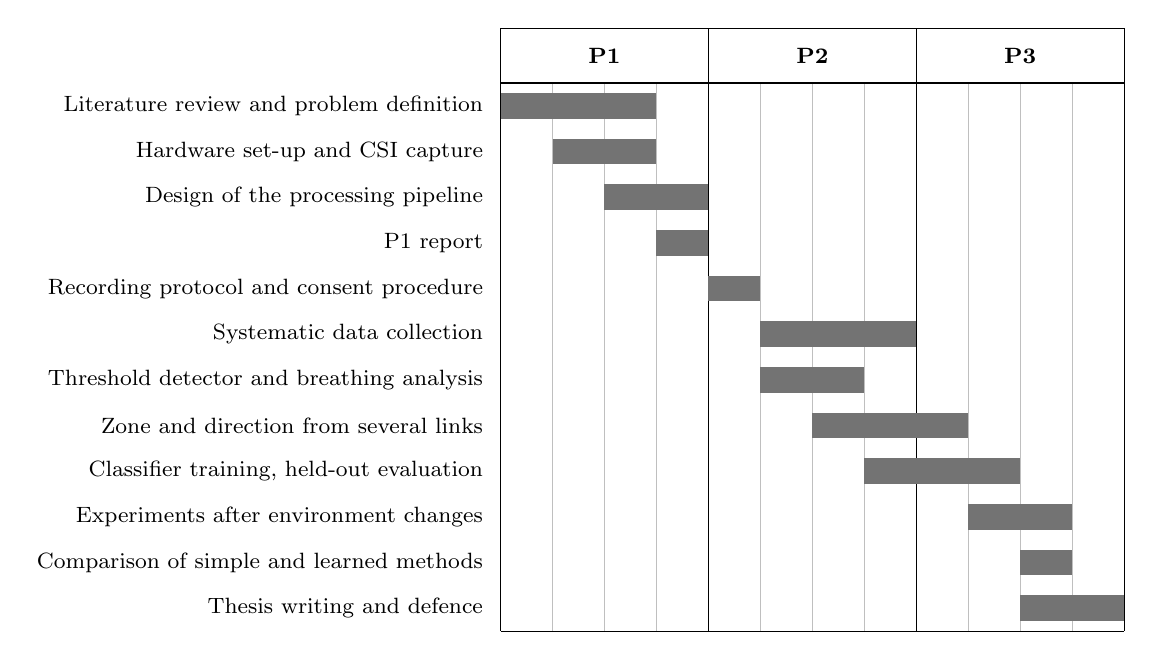
\begin{tikzpicture}[x=0.66cm, y=-0.58cm, font=\footnotesize]
  % header
  \foreach \s/\name in {0/P1, 4/P2, 8/P3} {
    \draw (\s,-1.2) rectangle (\s+4,0);
    \node at (\s+2,-0.6) {\textbf{\name}};
  }
  % grid
  \foreach \c in {0,...,12} \draw[black!25] (\c,0) -- (\c,12);
  \foreach \c in {0,4,8,12} \draw (\c,0) -- (\c,12);
  \draw (0,0) -- (12,0);
  \draw (0,12) -- (12,12);
  % tasks: row / start / end / name
  \foreach \row/\s/\e/\task in {
    0/0/3/{Literature review and problem definition},
    1/1/3/{Hardware set-up and CSI capture},
    2/2/4/{Design of the processing pipeline},
    3/3/4/{P1 report},
    4/4/5/{Recording protocol and consent procedure},
    5/5/8/{Systematic data collection},
    6/5/7/{Threshold detector and breathing analysis},
    7/6/9/{Zone and direction from several links},
    8/7/10/{Classifier training, held-out evaluation},
    9/9/11/{Experiments after environment changes},
    10/10/11/{Comparison of simple and learned methods},
    11/10/12/{Thesis writing and defence}} {
    \node[anchor=east] at (-0.15,\row+0.5) {\task};
    \fill[black!55] (\s,\row+0.22) rectangle (\e,\row+0.78);
  }
\end{tikzpicture}
\caption{Project timeline over the three thesis stages}
\label{fig:gantt}
\end{figure}

\section{Risk Management}
Table~\ref{tab:risk} lists the main risks of the project with their likelihood, their impact and the planned response. Most of them are technical and come from the limits of the hardware that were discussed in Section~\ref{sec:gap}.

{\small
\setlength{\tabcolsep}{4pt}
\begin{longtable}{L{3.4cm}L{2.1cm}L{1.5cm}L{6.4cm}}
\caption{Risks and planned responses}\label{tab:risk}\\
\toprule
\textbf{Risk} & \textbf{Likelihood} & \textbf{Impact} & \textbf{Planned response}\\
\midrule
\endfirsthead
\multicolumn{4}{l}{\small Table \thetable\ (continued)}\\
\toprule
\textbf{Risk} & \textbf{Likelihood} & \textbf{Impact} & \textbf{Planned response}\\
\midrule
\endhead
\bottomrule
\endfoot
A still person cannot be detected reliably from CSI amplitude alone & High & Medium & Treat the detection of a still person as an experimental result. Report the distances and positions in which it works and in which it fails. Movement detection remains the core result.\\\addlinespace
Accuracy drops when the room layout or the device placement changes & High & High & Repeat the empty-room calibration after every change. Describe the signal relative to the baseline. Measure the drop in separate experiments and report it.\\\addlinespace
Packet loss or an unsteady packet rate on one of the links & Medium & Medium & Keep the transmission rate fixed, time-stamp every packet, and leave out windows with too few packets.\\\addlinespace
Interference from other Wi-Fi devices or from people outside the room & Medium & Medium & Use a channel with little traffic, require agreement between links, and note the conditions of every session.\\\addlinespace
Too few labelled sessions or participants for the classifier & Medium & High & Fix the recording protocol early in P2, keep the number of classes small, and prefer simple models with few features.\\\addlinespace
Results look better than they are because training and test windows overlap & Medium & High & Split only by complete sessions. The split is done in one evaluation component that every experiment uses.\\\addlinespace
A device fails or devices behave differently & Low & Medium & Keep spare devices, use the same settings on all receivers, and document the placement with photographs.\\\addlinespace
Privacy concerns of the participants & Low & High & Ask for consent before every recording, store no names or images, and keep the recordings on the computers of the group.\\\addlinespace
The schedule slips & Medium & Medium & Give priority to presence and movement detection. Zone estimation and the classifier are extensions that can be reduced.\\
\end{longtable}
}
